\documentclass[a4paper, 10pt]{article}
\usepackage[T1]{fontenc}
\usepackage{multicol}
\usepackage{enumitem}
\usepackage{blindtext}
\usepackage{array}
\newcolumntype{P}[1]{>{\centering\arraybackslash}p{#1}}
\newcolumntype{M}[1]{>{\centering\arraybackslash}m{#1}}
\RequirePackage{lastpage}
\usepackage{hyperref}
\hypersetup{
	colorlinks=true,
	linkcolor=black,
	filecolor=magenta,      
	urlcolor=cyan,
	pdfpagemode=FullScreen,
}

%\pagenumbering{gobble}
%\pagenumbering{arabic}
%\usepackage{tgtermes}
%----------------------------------------------------------------------------------------
\usepackage{Alegreya} %% Option 'black' gives heavier bold face 
\renewcommand*\oldstylenums[1]{{\AlegreyaOsF #1}} %necessary to use Alegreya

%----------------------------------------------------------------------------------------
\usepackage[parfill]{parskip}
\usepackage{lipsum} % Un poco de texto de relleno
\usepackage{listings}
\usepackage{xcolor}
\usepackage{tcolorbox}
\usepackage{cascadia-code}
\lstloadlanguages{C,C++,csh,Java}

%Color scheme in Visual Studio darkmode
\definecolor{black}{cmyk}{0,0,0,1}             
\definecolor{white}{cmyk}{0,0,0,0}
\definecolor{darkgrey}{cmyk}{0,0,0,0.97}      %background in Visual Studio
\definecolor{green}{cmyk}{0.6,0,0.84,0}       %comments in Visual Studio
\definecolor{blue}{cmyk}{0.65,0.33,0,0.05}       %keywords in Visual Studio
\definecolor{rose}{cmyk}{0,0.26,0.38,0}       %strings in Visual Studio
\definecolor{lavender}{cmyk}{0,0.42,0,0.1}   %if/else,switch/case etc. in Visual Studio
\definecolor{lightblue}{cmyk}{0.35,0,0,0}     %local variables in Visual Studio
\definecolor{aqua}{cmyk}{0.65,0,0.23,0}       %class types in Visual Studio
\definecolor{lightgreen}{cmyk}{0.12,0,0.33,0.05} %enumerations and methods in Visual Studio

\lstset{
	language=[Sharp]C,
	basicstyle=\footnotesize\ttfamily,
	numbers=left, 
	numberstyle=\tiny\color{black}, 
	%rulesep=1pt,
	numbersep=1pt,
	tabsize=1,
	xleftmargin=1pt,
	framexleftmargin=-7pt,
	framexrightmargin=-5pt,
	showtabs=false,
	showspaces=false,
	showstringspaces=false,
	breaklines=true,
	breakatwhitespace=false,
	backgroundcolor=\color{darkgrey},
	rulecolor=\color{darkgrey},
	commentstyle=\color{green},
	morecomment=[s][\color{green}]{/*+}{*/},
	morecomment=[s][\color{green}]{/*-}{*/},
	basicstyle=\ttfamily\footnotesize\color{white},
	stringstyle=\color{rose},
	frame=trbl,
	framesep=5pt,
	numbersep=7pt,
	belowcaptionskip=1\baselineskip,
	%keywords like string, int, false, true ...
	keywordstyle=\color{blue},
	keywordstyle=[2]{\color{blue}},
	otherkeywords={var, value, get, set},
    morekeywords=[2]{var, predicate, page},
    %morekeywords=[2]{prueba},
	%-------------------------------------------
	%keywords like if/else, switch/cas ...
	emphstyle=\color{lavender},
	emph={if, else, return, throw, switch, case},
	%-------------------------------------------
	%Collection of your local and global variables
	emphstyle={[2]\color{lightblue}},
	emph={[2]someLocalVariable, someGlobalVariable},
	%-------------------------------------------
	%Collection of your class types
	emphstyle={[3]\color{aqua}},
	emph={[3]SomeOwnClassType},
	%-------------------------------------------
	%Collection of your methods
	emphstyle={[4]\color{lightgreen}},
	emph={[4]ToLower},
	}
	
\tcbuselibrary{listings,theorems,skins,vignette,raster,breakable,magazine,poster,fitting,hooks}

\usepackage{tikz}
\usepackage{tikzpagenodes}
\usetikzlibrary{calc}
\usetikzlibrary{mindmap}
\usepackage{lmodern}
\usepackage{atbegshi}
\usepackage{float}
%----------------------------------------------------------------------------------------
%	DOCUMENT MARGINS
%----------------------------------------------------------------------------------------
\usepackage{geometry}
\geometry{
	hmargin=1cm,
	bmargin=3cm,
	tmargin=4.5cm,
	centering
}

%----------------------------------------------------------------------------------------
\usepackage{tocloft}
\usepackage[explicit]{titlesec}

\usepackage{graphicx} % to add images 

\graphicspath{{images/}} % path to save the images

%\usepackage[abspage,user,lastpage]{zref}
%\makeatother

\definecolor{darkBlue}{RGB}{0,61,107}
\definecolor{skyBlue}{RGB}{21,190,240}
\definecolor{lightBlue}{RGB}{9,144,207}
\definecolor{lightGrey}{RGB}{188,190,192}
\definecolor{darkGrey}{RGB}{96,96,91}
\definecolor{backgroundGray}{RGB}{241,242,242}
\definecolor{oldJabilBlue}{RGB}{9,82,136}
\definecolor{textColor}{RGB}{65,64,66}
\definecolor{leafGreen}{RGB}{132,189,0}

\newcommand\Header{%
	\begin{tikzpicture}[remember picture,overlay]
		\fill[darkBlue]
		(current page.north west) -- (current page.north east) --
		([yshift=50pt]current page.north east|-current page text area.north east) --
		([yshift=50pt,xshift=-3cm]current page.north|-current page text area.north) --
		([yshift=10pt,xshift=-5cm]current page.north|-current page text area.north) --
		([yshift=10pt]current page.north west|-current page text area.north west) -- cycle;
		\node[font=\sffamily\bfseries\color{white},anchor=west,
		xshift=0.5cm,yshift=-1.2cm] at (current page.north west)
		{\fontsize{30}{40}\selectfont Estándar de Desarrollo};
		\node[xshift=-4.5cm,yshift=-1cm] (myfirstpic) at (current page.north east) {
\includegraphics[width=6cm]{jabilLogo2}};
		\node[xshift=-5cm,yshift=-2cm] (secondpic) at (current page.north east) {
\includegraphics[width=5cm]{jabilLogo4}};
	\end{tikzpicture}%
}
\newcommand\Footer{%
	\begin{tikzpicture}[remember picture,overlay]
		\fill[darkBlue]
		(current page.south west) -- (current page.south east) --
		([yshift=-40pt]current page.south east|-current page text area.south east) --
		([yshift=-40pt,xshift=-3cm]current page.south|-current page text area.south) --
		([xshift=-5cm,yshift=-10pt]current page.south|-current page text area.south) --
		([yshift=-10pt]current page.south west|-current page text area.south west) -- cycle;
		\node[yshift=0.75cm,font=\ttfamily\bfseries\color{white}] at (current page.south) {\fontsize{10}{14}\selectfont CONFIDENTIAL AND PROPIETARY};
		\node[xshift=3cm, yshift=0.75cm,font=\ttfamily\bfseries\color{white}] at (current page.south west) {\fontsize{10}{14}\selectfont Equipo de desarrollo de MFG};
		\node[xshift=-3cm, yshift=0.75cm,font=\ttfamily\bfseries\color{white}] at (current page.south east) {\fontsize{10}{14}\selectfont };
		\node[font=\sffamily\bfseries\color{white},anchor=west,
		xshift=0.5cm,yshift=-1.2cm] at (current page.north west)
		{\fontsize{50}{60}\selectfont };
	\end{tikzpicture}%
}

\pagestyle{empty}
\AtBeginShipout{\Header\Footer}
\AtBeginShipoutFirst{\Header\Footer}

\renewcommand*\thesection{\arabic{section}}
%\renewcommand*\thesection{\arabic{sectiontc}}

\definecolor{myBlue}{HTML}{0088FF}


\titleformat{\section}[hang]{\Large\bfseries\sffamily}%
{\rlap{\color{darkBlue}\rule[-6pt]{\columnwidth}{2pt}}\colorbox{darkBlue}{%
		\raisebox{0pt}[13pt][3pt]{ \makebox[60pt]{% height, width
				\fontfamily{phv}\selectfont\color{white}{\thesection}}
}}}%
{15pt}%
{ \color{darkBlue}#1
	%
}

\titleformat{\subsection}[hang]{\large\bfseries\sffamily}%
{\rlap{\color{lightBlue}\rule[-6pt]{\columnwidth}{1.5pt}}\colorbox{lightBlue}{%
		\raisebox{0pt}[10pt][2pt]{ \makebox[50pt]{% height, width
				\fontfamily{phv}\selectfont\color{white}{\thesubsection}}
}}}%
{15pt}%
{ \color{lightBlue}#1
	%
}

\titleformat{\contents}[hang]{\large\bfseries\sffamily}%
{\rlap{\color{lightBlue}\rule[-6pt]{\columnwidth}{1.5pt}}\colorbox{lightBlue}{%
		\raisebox{0pt}[10pt][2pt]{ \makebox[50pt]{% height, width
				\fontfamily{phv}\selectfont\color{white}{\thesubsection}}
}}}%
{15pt}%
{ \color{lightBlue}#1
	%
}

\titlespacing*{\section}{0pt}{3mm}{5mm}
\titlespacing*{\subsection}{0pt}{3mm}{5mm}
\usepackage{titletoc}

\newlength{\tocsep} 
\setlength\tocsep{1.5pc} % Sets the indentation of the sections in the table of contents
\setcounter{tocdepth}{3} % Three levels in the table of contents section: sections, subsections and subsubsections

\usepackage{titletoc}
\contentsmargin{0cm}

\titlecontents{section}[\tocsep]
{\addvspace{4pt}\small\bfseries\sffamily}
{\contentslabel[\thecontentslabel]{\tocsep}}
{}
{\ \titlerule*[.5pc]{.}\ \thecontentspage}
[]

\titlecontents{subsection}[\tocsep]
{\addvspace{2pt}\sffamily}
{\contentslabel[\thecontentslabel]{\tocsep}}
{}
{\ \titlerule*[.5pc]{.}\ \thecontentspage}
[]

\titlecontents*{subsubsection}[\tocsep]
{\footnotesize\sffamily}
{}
{}
{}
[\ \textbullet\ ]

%----------------------------------------------------------------------------------------
%	DOCUMENT MARGINS
%----------------------------------------------------------------------------------------
\DeclareTotalTCBox{\commandbox}{ s v }
{verbatim,colupper=white,colback=black!75!white,colframe=black}
{\IfBooleanT{#1}{\textcolor{red}{\ttfamily\bfseries > }}%
	\lstinline[language=command.com,keywordstyle=\color{blue!35!white}\bfseries]^#2^}
%----------------------------------------------------------------------------------------
\renewcommand{\contentsname}{Contenido}
\begin{document}
\clearpage

\begin{tcolorbox}[colback=white!5!white, colframe=lightGrey, boxrule=0.3mm, arc=0mm, boxsep=0mm, left=1mm, right=1mm, bottom=1mm, top=1mm]
	\begin{tcolorbox}[colback=backgroundGray, colframe=white, arc=0mm, fontupper=\color{textColor}\sffamily\bfseries]
		\large Abstracto\\\\
		\normalsize El objetivo del presente documento es el de brindar las bases importantes, bases que se deben de tomar en cuenta para el desarrollo de las aplicaciones, desde la realización de la documentación hasta la finalización del desarrollo. Se establecerán las reglas para los 3 esquemas que se manejan actualmente: Base de Datos, Back-end y Front-end.
	\end{tcolorbox}%
\end{tcolorbox}


\begin{multicols}{2}
\tableofcontents


\section{BackEnd}

A continuación se establecen los puntos que el desarrollador debe tomar en cuenta para la implementación, ya sea de proyectos nuevos, refactorizaciones o agregar nuevas características a proyectos existentes.


\subsection{Etapa de desarrollo}

\begin{itemize}
\item Cuando se trate de un \textbf{proyecto nuevo}, el desarrollador deberá tener iniciado el \sffamily TSD \normalfont y tener iniciado el \sffamily USR, \normalfont al menos con los datos importantes del proyecto. El desarrollador deberá guardarlos en la carpeta de la documentación (sharepoint) junto con el \sffamily BRD \normalfont y el \sffamily TSD \normalfont y deberá mandar un correo a \href{mailto:me@example.com}{joel\_castillejos3@jabil.com} solicitando la creación del repositorio adjuntando la URL del repositorio de documentos y el nombre del repositorio a crear. El repositorio deberá tener una nomenclatura similar a este ejemplo: BreakoutPanelAndScrap.Americas.GTP\\

\begin{figure}[H]
	\centering
	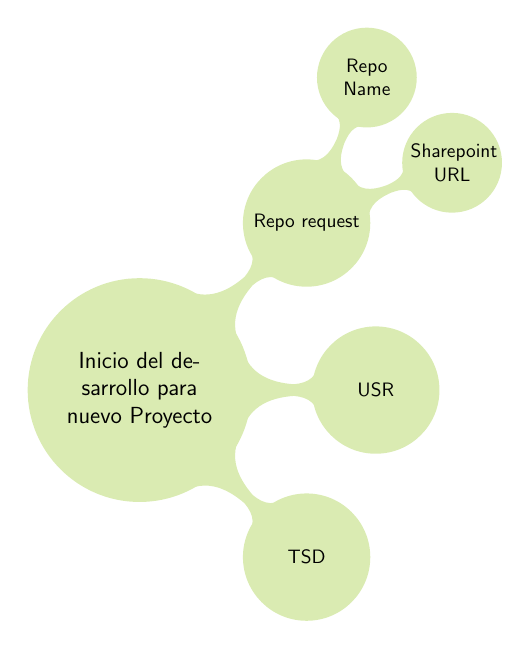
\begin{tikzpicture}[mindmap, every node/.style=concept, concept color=leafGreen!30,
		grow cyclic,
		level 1/.append style={level distance=3cm,sibling angle=45},
		level 2/.append style={level distance=2cm,sibling angle=45},
		level 3/.append style={level distance=2cm,sibling angle=45}]
		\tikzset{every node/.append style={scale=0.7,font=\sffamily}}
		\node [root concept] {\sffamily Inicio del desarrollo para nuevo Proyecto}
		child { node {TSD}}
		child { node {USR}}
		child { node {Repo request}
			child { node {Sharepoint URL}}
			child { node {Repo Name}}
	};
			
	\end{tikzpicture}
\end{figure} 
\item Cuando se trate de agregar características a un proyecto se debe generar la parte inicial del \sffamily TSD \normalfont y agregarlo en el sharepoint con la nueva versión del proyecto a mejora (dentro del sharepoint el BSA a cargo debe de crear una carpeta con el nombre de la versión correspondiente).

\item Para las remediaciones de código se deberá generar el \sffamily IT Form Control Change \normalfont y agregarlo a la carpeta correspondiente del proyecto.

\item Para establecer un manejo adecuado de las ramas, siempre deberá crear la rama \sffamily“development” \normalfont a partir de \sffamily“master” \normalfont y todas las nuevas características o remediaciones deberán partir de la rama \sffamily“development” \normalfont.

\item Cuando se termine una remediación o una nueva característica se creará un \sffamily“Pull Request” \normalfont hacia development pidiendo por correo la revisión de código adjuntando la URL del Pull Request, el formato del \sffamily Code Peer Review, \normalfont la rama \sffamily feature/hotfix \normalfont deberá ser borrada una vez aprobado y completado el Pull Request.
\end{itemize}
\end{multicols}	

\newpage
\begin{itemize}
	\item Toda cadena de conexión deberá ser encriptada con la ayuda de la herramienta \href{}{JabilEncryptor} y se establecerá el valor de de \texttt{IsEncrypted} en \texttt{True}.
	
	\item Cuando se trate de un proyecto con arquitectura \sffamily Rest Api \normalfont (Api con JabilCore) se deberá configurar las cadenas de conexión en los 3 ambientes: \sffamily Development, Staging y Prodduction.\normalfont En cuanto a producción, el BSA nos deberá proporcinar en qué servidor se estará subiendo la aplicación.
	
	\item Cuando se trate de un proyecto con arquitectura \sffamily Rest \normalfont (Api con JabilCore) se deberá configurar la sección "JabilCore" en los 3 ambientes: Development (ya se encuentra configurado), Staging (el desarrollador establecerá el servidor y la estructura de carpteas) y Production (el BSA deberá proporcionar el nombre del servidor y el desarrollador establecerá la misma estructura de carpetas).
	
	\item Al finalizar un proyecto, el desarrollador tendrá que generar el manual de instalación en caso de que no se cuente con uno.
	
	\item Para los proyectos \sffamily Rest \normalfont (Api con JabilCore) los controladores deberán de estar lo más limpios posibles, es decir, tener el llamado al servicio y a lo mucho establecer el usuario que está haciendo la petición.
	
	\item Toda llamada del servicio en el controlador deberá estar dentro de una respuesta \sffamily Ok \normalfont como se muestra a continuación.
	\begin{lstlisting}[language={[Sharp]C}]
	[HttpGet"({page}/{pageSize}/{predicate}/{sort}/{sortDirection}"), ActionName("GetSites"), Logging]
	public IActionResult GetSites(int page, int pageSize, string predicate, string sort, string sortDirection)
	{
		var prueba = HttpContext.User.Identity.Name;
		return Ok(this._SiteRetrieveService.RetrieveResultWhere(predicate, page, pageSize, sort, sortDirection, null);
	}
	\end{lstlisting}

	\item Todo servicio llamado desde un \sffamily ProcessService, RetrieveService o WriteService \normalfont debe ser verificado para determinar si se ejecutó de forma adecuada.
	\begin{lstlisting}[language={[Sharp]C}]
	var nameResult = this._BuildingRetrieveService.RetrieveResultWhere(p => p.Name.ToLower().Equals(this._Entity.Name.ToLower())
	p.SiteId == this._Entity.SiteId);
	if (nameResult.Fail throw new OperationCanceledException(nameResult.GetMessage()); 
	\end{lstlisting}
	
	\item Todos los nombres de los métodos deben tener la nomenclatura \sffamily PascalCase \normalfont y será nombrado en inglés.
	
	\item Todo comentario explicativo deberá ser en inglés
	
	\item Las entidades deberán cumplir con la nomenclatura \sffamily PascalCase \normalfont sin llevar algún caracter especial. en caso de que la tabla tenga una nomenclatura diferente en .NET deberá hacerse uso de las \sffamily DataNotation \normalfont para hacerlas coincidir.
	
	\item Para la validación de los registros en los procesos de escritura, deberán ser agregados en los métodos \sffamily ValidateCreate y ValidateUpdate \normalfont como se muestra a continuación.
	
	\begin{lstlisting}[language={[Sharp]C}]
		public overrride bool ValidateCreate()
		{
			var nameResult = this._BuildingRetrieveService.RetrieveResultWhere(p => p.Name.ToLower().Equals(this._Entity.Name.Tolower() && p.SiteId == this._Entity.SiteId);
			if (nameResult.Fail) throw new OperationCanceledException(nameResult.GetMessage());
			
			if (nameResult.Data.ToList().Count > 0) throw new SystemValidationExcepton("BUILDING.NAME_ALREADY_EXISTS");
			
			return true;		
		}
		
		public override bool ValidateUpdate()
		{
			var nameResult = this._BuildingRetrieveService.RetrieveResultWhere(p => p.Id != this._Entity.Id && p.Name.ToLower().Equals)
			if (!nameResult.Success) throw new OperationCanceledException(nameResult.GetMessage());
			
			if (nameResult.Data.ToList.Count > 0) throw new SystemValidationExcepton("BUILDING.NAME_ALREADY_EXISTS");
		}
	\end{lstlisting}
	
	\item Respecto a la regla de los procesos, los \sffamily RetrieveService \normalfont sólo pueden llamar a otros \sffamily RetrieveService, \normalfont los \sffamily WriteService \normalfont sólo pueden llamar a otros \sffamily RetrieveService o WriteService \normalfont y los \sffamily ProcessService \normalfont pueden ejecutar cualquiera de los tres servicios.
	
	\begin{figure}[H]
		\centering
		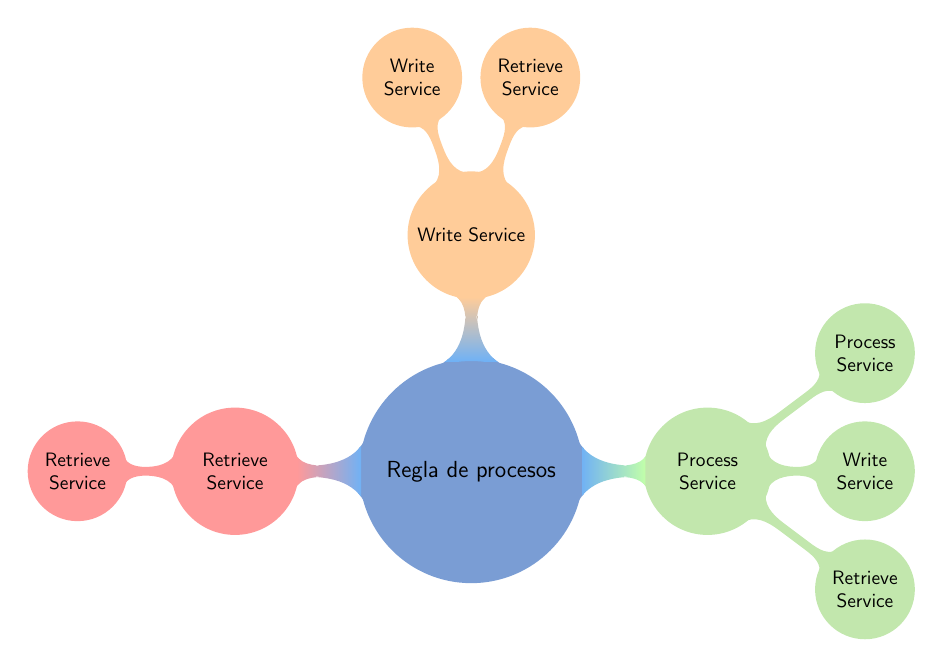
\begin{tikzpicture}[mindmap, every node/.style=concept, concept color=blue!80,
			grow cyclic,
			level 1/.append style={level distance=3cm,sibling angle=60},
			level 2/.append style={level distance=2cm,sibling angle=45},
			level 3/.append style={level distance=2cm,sibling angle=45},
			]
			\tikzset{every node/.append style={scale=0.7,font=\sffamily}}
			\node [root concept] {\sffamily Regla de procesos}
			child[concept color=red!40, grow=180] { node {Retrieve Service}
				child {node {Retrieve Service}}
			}
			child[concept color=orange!40, grow=90] { node {Write Service}
				child {node {Retrieve Service}}
				child {node {Write Service}}
			}
			child[concept color=green!40, grow=0] { node {Process Service}
				child { node {Retrieve Service}}
				child { node {Write Service}}
				child { node {Process Service}}
			};
			
		\end{tikzpicture}
	\end{figure} 
	\item Cuando un proceso lleve demasiadas líneas de código o demasiada lógica o llamado a otros servicios entonces se deberá usar un \sffamily ProcessService \normalfont de forma obligatoria.
	
	\item Todo código comentado deberá ser borrado.
	
	\item Las enumeraciones deben estar en el proyecto de \sffamily Models \normalfont dentro de una carpeta llamada  \sffamily Enumerations, \normalfont los \sffamily DTO \normalfont deberán estar en una carpeta llamada \sffamily DTOs \normalfont dentro de \sffamily Models \normalfont y las clases parciales que extienden a los modelos deberán estar en una carpeta llamada \sffamily Partials \normalfont.
	
\end{itemize}

\begin{multicols}{2}
\section{Front End}
A continuación se establecen los puntos que el desarrollador debe tomar en cuenta para su desarrollo con interfaces de usuario, ya sea con \sffamily MVC Razon, Angular o ASP.NET \normalfont.

\begin{itemize}
	\item Cuando se requiera diseñar pantallas de un proyecto existente, el desarrollador deberá tomar en cuenta las pantallas existentes, para saber qué componentes y estructuras está usando.
	\item Cuando sea una aplicación nueva se tomará como ejemplo los mock ups presentados por el BSA, el desarollador puede proponer ajustes al estilo.
	\item Al utilizar la plantilla Angular de Jabil todos los catálogos deberán llevar el mismo formato que el componente de ejemplo, llamado \texttt{console-component}.
	
	\item Si se utiliza la plantilla de Angular de Jabil deberá configurarse desde un principio los archivos \sffamily index \normalfont de cada ambiente.
	\item En caso de utilizar alguna autenticación como Okta/Cognito, el desarrollador deberá realizar las pruebaas necesarias para el ambiente de producción.
	\item Los métodos en TypeScript debe utilizar la notación \sffamily lower camel case \normalfont .
\end{itemize}
\end{multicols}

\begin{itemize}
		\item Es obligatorio utilizar servicios para comunicarse con las APIs al utilizar la plantilla de Angular.
		
		\item Todas las entidades deberás ser mapeadas como interfaces o clases en Angular para forzar el tipado.
		
		\item No repetir nombres claves para las llaves en los archivos de traducción.
		
		\item Sólo se permite un nivel de anidación:
		\begin{lstlisting}[language={[Sharp]C}]
		"HOME": {
				"TITLE": "Hello Translate!",
				"SELECT_LANGUAGE": "Change Language",
				"ALERTS": "Alerts",
				"HELP": "Help"
		},
		"NAV": {
				"APPLICATIONS": "Application",
				"CATALOGS": "Catalogs",
				"CONSOLES": "Consoles"
		},
		"ERRORS":{
				"NOT_FOUND": "PAGE NOT FOUND",
				"DEFAULT": "There was an error in the application..."
		}
		\end{lstlisting}
		
\end{itemize}

\section{Referencias a documentos y conexiones}

\subsection{Referencias}

	\begin{table}[H]
		\centering
		\begin{tabular}{|M{5cm}|M{10cm}|}
			\hline
			Documento / App & Link  \\ \hline
			TSD                 & \href{https://teams.microsoft.com/l/message/48:notes/1709515023086?context=%7B%22contextType%22%3A%22chat%22%7D}{TSD Thecnical Specification Document - Template}   \\ \hline
			Code Peer Review                      & \href{https://jabil.sharepoint.com/:x:/r/sites/GTPDevelopementTeam/_layouts/15/Doc.aspx?sourcedoc=%7B07743DB1-7477-4074-A4A2-4FC4EB709F03%7D&file=PeerReview%20template.xlsm&wdLOR=c9D6048F5-053F-4B75-B430-3EF5F6F05533&action=default&mobileredirect=true}{Peer Review Template}   \\ \hline
			IT Form Control Change                   & \href{https://jabil.sharepoint.com/:x:/r/sites/GTPDevelopementTeam/_layouts/15/Doc.aspx?sourcedoc=%7B804A211B-F279-4C3F-AF61-67B43529AC11%7D&file=IT-FormControlChange%20-%20Template.xlsx&wdLOR=cCCF118CB-F307-4DB1-A55C-20D350358B63&action=default&mobileredirect=true}{IT Form Control Change - Template}  \\ \hline
			Jabil Encryptor &  \href{https://dev.azure.com/jblprd/EMS%20Applications/_git/JBCore.Americas.GTP?path=/Resources/JabilEncryptor.zip}{JabilEncryptor.zip - Repos (Azure)}  \\ \hline
			USR & \href{https://jabil.sharepoint.com/:x:/r/sites/InfrastructureandOperationsEnablementsSDLC/_layouts/15/Doc.aspx?sourcedoc=%7B71142002-4CFD-4282-BEC1-9B5D37D2C810%7D&file=USR%20Assessment%20template.xlsm&wdLOR=c08DF94E0-411D-472F-9012-C6B62DF8692A&action=default&mobileredirect=true}{USR -Template}  \\ \hline
		\end{tabular}
		\newline\newline
	\end{table}

\subsection{Conexiones}

RDS Postgres
\begin{itemize}
	\item Producción
	\begin{lstlisting}[language={[Sharp]C}]
		Instancia de Lectura: "rds00-475137724643-ehsdg-001-instance-1-us-east-1a.c0lgirv4jfz4.us-east-1.rds.amazonaws.com"
		Instancia de escritura: "rds00-475137724643-ehsdg-001-instance-1-us-east-1b.c0lgirv4jfz4.us-east-1.rds.amazonaws.com"
	\end{lstlisting}
	
	\item Desarrollo
	\begin{lstlisting}[language={[Sharp]C}]
		"rds-50354-00029-emsmxgdl-001.cluster-c3djzrupnnjg.us-east-1.rds.amazonaws.com
		"
	\end{lstlisting}

\end{itemize}

 Rabbit
\begin{lstlisting}[language={[Sharp]C}]
	"JabilLoggin": {
		"Host": "awuwe2web82",
		"UserName": "jlogging",
		"Password": "JabilLogging2348",
		"Port": 5672
	}
\end{lstlisting}
\end{document}